% GNUPLOT: LaTeX picture with Postscript
\begingroup
  \makeatletter
  \providecommand\color[2][]{%
    \GenericError{(gnuplot) \space\space\space\@spaces}{%
      Package color not loaded in conjunction with
      terminal option `colourtext'%
    }{See the gnuplot documentation for explanation.%
    }{Either use 'blacktext' in gnuplot or load the package
      color.sty in LaTeX.}%
    \renewcommand\color[2][]{}%
  }%
  \providecommand\includegraphics[2][]{%
    \GenericError{(gnuplot) \space\space\space\@spaces}{%
      Package graphicx or graphics not loaded%
    }{See the gnuplot documentation for explanation.%
    }{The gnuplot epslatex terminal needs graphicx.sty or graphics.sty.}%
    \renewcommand\includegraphics[2][]{}%
  }%
  \providecommand\rotatebox[2]{#2}%
  \@ifundefined{ifGPcolor}{%
    \newif\ifGPcolor
    \GPcolortrue
  }{}%
  \@ifundefined{ifGPblacktext}{%
    \newif\ifGPblacktext
    \GPblacktexttrue
  }{}%
  % define a \g@addto@macro without @ in the name:
  \let\gplgaddtomacro\g@addto@macro
  % define empty templates for all commands taking text:
  \gdef\gplbacktext{}%
  \gdef\gplfronttext{}%
  \makeatother
  \ifGPblacktext
    % no textcolor at all
    \def\colorrgb#1{}%
    \def\colorgray#1{}%
  \else
    % gray or color?
    \ifGPcolor
      \def\colorrgb#1{\color[rgb]{#1}}%
      \def\colorgray#1{\color[gray]{#1}}%
      \expandafter\def\csname LTw\endcsname{\color{white}}%
      \expandafter\def\csname LTb\endcsname{\color{black}}%
      \expandafter\def\csname LTa\endcsname{\color{black}}%
      \expandafter\def\csname LT0\endcsname{\color[rgb]{1,0,0}}%
      \expandafter\def\csname LT1\endcsname{\color[rgb]{0,1,0}}%
      \expandafter\def\csname LT2\endcsname{\color[rgb]{0,0,1}}%
      \expandafter\def\csname LT3\endcsname{\color[rgb]{1,0,1}}%
      \expandafter\def\csname LT4\endcsname{\color[rgb]{0,1,1}}%
      \expandafter\def\csname LT5\endcsname{\color[rgb]{1,1,0}}%
      \expandafter\def\csname LT6\endcsname{\color[rgb]{0,0,0}}%
      \expandafter\def\csname LT7\endcsname{\color[rgb]{1,0.3,0}}%
      \expandafter\def\csname LT8\endcsname{\color[rgb]{0.5,0.5,0.5}}%
    \else
      % gray
      \def\colorrgb#1{\color{black}}%
      \def\colorgray#1{\color[gray]{#1}}%
      \expandafter\def\csname LTw\endcsname{\color{white}}%
      \expandafter\def\csname LTb\endcsname{\color{black}}%
      \expandafter\def\csname LTa\endcsname{\color{black}}%
      \expandafter\def\csname LT0\endcsname{\color{black}}%
      \expandafter\def\csname LT1\endcsname{\color{black}}%
      \expandafter\def\csname LT2\endcsname{\color{black}}%
      \expandafter\def\csname LT3\endcsname{\color{black}}%
      \expandafter\def\csname LT4\endcsname{\color{black}}%
      \expandafter\def\csname LT5\endcsname{\color{black}}%
      \expandafter\def\csname LT6\endcsname{\color{black}}%
      \expandafter\def\csname LT7\endcsname{\color{black}}%
      \expandafter\def\csname LT8\endcsname{\color{black}}%
    \fi
  \fi
  \setlength{\unitlength}{0.0500bp}%
  \begin{picture}(8500.00,8500.00)%
    \gplgaddtomacro\gplbacktext{%
      \colorrgb{0.70,0.70,0.70}%
      \put(951,4845){\makebox(0,0)[r]{\strut{} 0}}%
      \colorrgb{0.70,0.70,0.70}%
      \put(951,5619){\makebox(0,0)[r]{\strut{} 0.005}}%
      \colorrgb{0.70,0.70,0.70}%
      \put(951,6393){\makebox(0,0)[r]{\strut{} 0.01}}%
      \colorrgb{0.70,0.70,0.70}%
      \put(951,7167){\makebox(0,0)[r]{\strut{} 0.015}}%
      \colorrgb{0.70,0.70,0.70}%
      \put(951,7941){\makebox(0,0)[r]{\strut{} 0.02}}%
      \colorrgb{0.70,0.70,0.70}%
      \put(1053,4659){\makebox(0,0){\strut{} 0}}%
      \colorrgb{0.70,0.70,0.70}%
      \put(2093,4659){\makebox(0,0){\strut{} 15}}%
      \colorrgb{0.70,0.70,0.70}%
      \put(3133,4659){\makebox(0,0){\strut{} 30}}%
      \colorrgb{0.70,0.70,0.70}%
      \put(4173,4659){\makebox(0,0){\strut{} 45}}%
      \colorrgb{0.70,0.70,0.70}%
      \put(5213,4659){\makebox(0,0){\strut{} 60}}%
      \colorrgb{0.70,0.70,0.70}%
      \put(6253,4659){\makebox(0,0){\strut{} 75}}%
      \colorrgb{0.70,0.70,0.70}%
      \put(7293,4659){\makebox(0,0){\strut{} 90}}%
      \put(7395,4845){\makebox(0,0)[l]{\strut{}-20}}%
      \put(7395,5619){\makebox(0,0)[l]{\strut{}-19.5}}%
      \put(7395,6393){\makebox(0,0)[l]{\strut{}-19}}%
      \put(7395,7167){\makebox(0,0)[l]{\strut{}-18.5}}%
      \put(7395,7941){\makebox(0,0)[l]{\strut{}-18}}%
      \csname LTb\endcsname%
      \put(144,6393){\rotatebox{-270}{\makebox(0,0){\strut{}Transmission Coefficient Magnitude}}}%
      \csname LTb\endcsname%
      \put(8099,6393){\rotatebox{-270}{\makebox(0,0){\strut{}Transmission Coefficient Phase}}}%
      \csname LTb\endcsname%
      \put(4173,4380){\makebox(0,0){\strut{}Angle [degrees]}}%
      \put(4173,8220){\makebox(0,0){\strut{}Angle vs Transmission Coefficient (At Five Skin Depths)}}%
    }%
    \gplgaddtomacro\gplfronttext{%
      \csname LTb\endcsname%
      \put(6505,7774){\makebox(0,0)[r]{\strut{}Magnitude}}%
      \csname LTb\endcsname%
      \put(6505,7588){\makebox(0,0)[r]{\strut{}Phase}}%
    }%
    \gplgaddtomacro\gplbacktext{%
      \colorrgb{0.70,0.70,0.70}%
      \put(951,595){\makebox(0,0)[r]{\strut{} 0.98}}%
      \colorrgb{0.70,0.70,0.70}%
      \put(951,1369){\makebox(0,0)[r]{\strut{} 0.985}}%
      \colorrgb{0.70,0.70,0.70}%
      \put(951,2144){\makebox(0,0)[r]{\strut{} 0.99}}%
      \colorrgb{0.70,0.70,0.70}%
      \put(951,2918){\makebox(0,0)[r]{\strut{} 0.995}}%
      \colorrgb{0.70,0.70,0.70}%
      \put(951,3692){\makebox(0,0)[r]{\strut{} 1}}%
      \colorrgb{0.70,0.70,0.70}%
      \put(1053,409){\makebox(0,0){\strut{} 0}}%
      \colorrgb{0.70,0.70,0.70}%
      \put(2059,409){\makebox(0,0){\strut{} 15}}%
      \colorrgb{0.70,0.70,0.70}%
      \put(3065,409){\makebox(0,0){\strut{} 30}}%
      \colorrgb{0.70,0.70,0.70}%
      \put(4071,409){\makebox(0,0){\strut{} 45}}%
      \colorrgb{0.70,0.70,0.70}%
      \put(5077,409){\makebox(0,0){\strut{} 60}}%
      \colorrgb{0.70,0.70,0.70}%
      \put(6083,409){\makebox(0,0){\strut{} 75}}%
      \colorrgb{0.70,0.70,0.70}%
      \put(7089,409){\makebox(0,0){\strut{} 90}}%
      \put(7191,595){\makebox(0,0)[l]{\strut{} 179}}%
      \put(7191,1369){\makebox(0,0)[l]{\strut{} 179.25}}%
      \put(7191,2144){\makebox(0,0)[l]{\strut{} 179.5}}%
      \put(7191,2918){\makebox(0,0)[l]{\strut{} 179.75}}%
      \put(7191,3692){\makebox(0,0)[l]{\strut{} 180}}%
      \csname LTb\endcsname%
      \put(144,2143){\rotatebox{-270}{\makebox(0,0){\strut{}Reflection Coefficient Magnitude}}}%
      \csname LTb\endcsname%
      \put(8099,2143){\rotatebox{-270}{\makebox(0,0){\strut{}Reflection Coefficient Phase}}}%
      \csname LTb\endcsname%
      \put(4071,130){\makebox(0,0){\strut{}Angle [degrees]}}%
      \put(4071,3971){\makebox(0,0){\strut{}Angle vs Reflection Coefficient (At Five Skin Depths)}}%
    }%
    \gplgaddtomacro\gplfronttext{%
      \csname LTb\endcsname%
      \put(6301,2236){\makebox(0,0)[r]{\strut{}Magnitude}}%
      \csname LTb\endcsname%
      \put(6301,2050){\makebox(0,0)[r]{\strut{}Phase}}%
    }%
    \gplbacktext
    \put(0,0){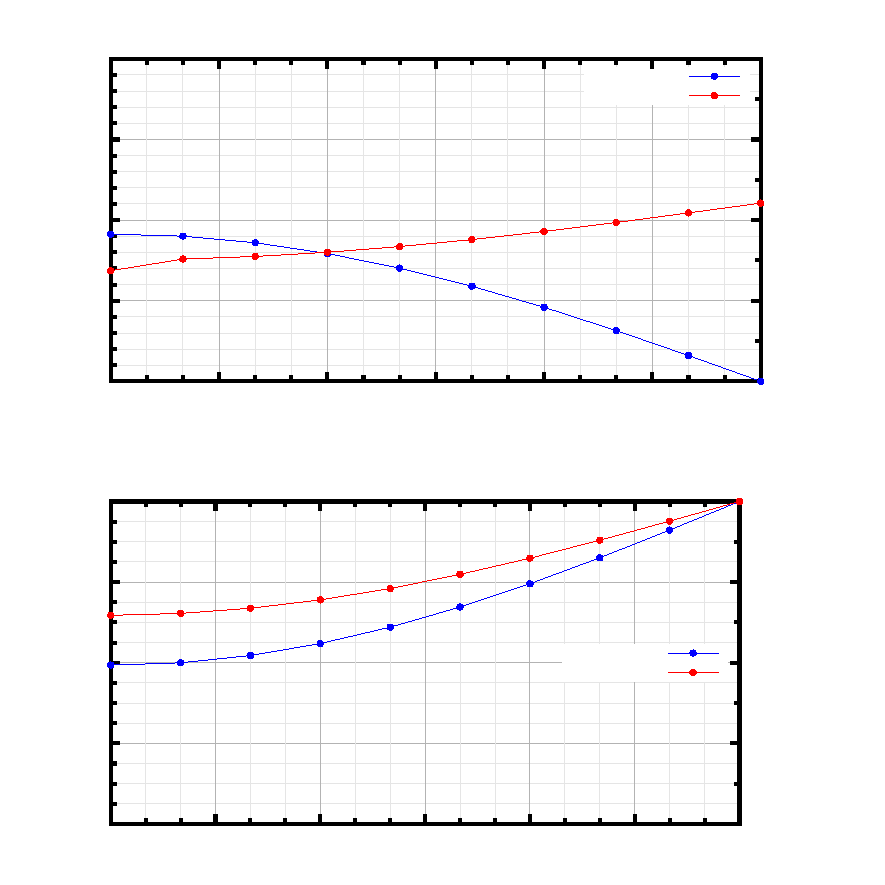
\includegraphics{../Code/11cTRAngle_Plot/11cTRAngle}}%
    \gplfronttext
  \end{picture}%
\endgroup
